\documentclass[journal,12pt,twocolumn]{IEEEtran}

\usepackage{setspace}
\usepackage{gensymb}


\singlespacing

\usepackage[cmex10]{amsmath}
%\usepackage{amsthm}
%\interdisplaylinepenalty=2500
%\savesymbol{iint}
%\usepackage{txfonts}
%\restoresymbol{TXF}{iint}
%\usepackage{wasysym}
\usepackage{amsthm}

\usepackage{mathrsfs}
\usepackage{txfonts}
\usepackage{stfloats}
\usepackage{bm}
\usepackage{cite}
\usepackage{cases}
\usepackage{subfig}

\usepackage{longtable}
\usepackage{multirow}

\usepackage{enumitem}
\usepackage{mathtools}
\usepackage{steinmetz}
\usepackage{tikz}
\usepackage{circuitikz}
\usepackage{verbatim}
\usepackage{tfrupee}
\usepackage[breaklinks=true]{hyperref}

\usepackage{tkz-euclide} %loads TikZ and tkz-base

\usetikzlibrary{calc,math}
\usepackage{listings}
    \usepackage{color}                                          
    \usepackage{array}                                          
    \usepackage{longtable}                                      
    \usepackage{calc}                                          
    \usepackage{multirow}                                      
    \usepackage{hhline}                                        
    \usepackage{ifthen}
    \usepackage{lscape}    
\usepackage{multicol}
\usepackage{chngcntr}

\DeclareMathOperator*{\Res}{Res}

\renewcommand\thesection{\arabic{section}}
\renewcommand\thesubsection{\thesection.\arabic{subsection}}
\renewcommand\thesubsubsection{\thesubsection.\arabic{subsubsection}}

\renewcommand\thesectiondis{\arabic{section}}
\renewcommand\thesubsectiondis{\thesectiondis.\arabic{subsection}}
\renewcommand\thesubsubsectiondis{\thesubsectiondis.\arabic{subsubsection}}

\hyphenation{op-tical net-works semi-conduc-tor}
\def\inputGnumericTable{}                                 %%

\lstset{
%language=C,
frame=single,
breaklines=true,
columns=fullflexible
}

\begin{document}

\newtheorem{theorem}{Theorem}[section]
\newtheorem{problem}{Problem}
\newtheorem{proposition}{Proposition}[section]
\newtheorem{lemma}{Lemma}[section]
\newtheorem{corollary}[theorem]{Corollary}
\newtheorem{example}{Example}[section]
\newtheorem{definition}[problem]{Definition}

\newcommand{\BEQA}{\begin{eqnarray}}
\newcommand{\EEQA}{\end{eqnarray}}
\newcommand{\define}{\stackrel{\triangle}{=}}
\bibliographystyle{IEEEtran}
\providecommand{\mbf}{\mathbf}
\providecommand{\pr}[1]{\ensuremath{\Pr\left(#1\right)}}
\providecommand{\qfunc}[1]{\ensuremath{Q\left(#1\right)}}
\providecommand{\sbrak}[1]{\ensuremath{{}\left[#1\right]}}
\providecommand{\lsbrak}[1]{\ensuremath{{}\left[#1\right.}}
\providecommand{\rsbrak}[1]{\ensuremath{{}\left.#1\right]}}
\providecommand{\brak}[1]{\ensuremath{\left(#1\right)}}
\providecommand{\lbrak}[1]{\ensuremath{\left(#1\right.}}
\providecommand{\rbrak}[1]{\ensuremath{\left.#1\right)}}
\providecommand{\cbrak}[1]{\ensuremath{\left\{#1\right\}}}
\providecommand{\lcbrak}[1]{\ensuremath{\left\{#1\right.}}
\providecommand{\rcbrak}[1]{\ensuremath{\left.#1\right\}}}
\theoremstyle{remark}
\newtheorem{rem}{Remark}
\newcommand{\sgn}{\mathop{\mathrm{sgn}}}
\providecommand{\abs}[1]{\left\vert#1\right\vert}
\providecommand{\res}[1]{\Res\displaylimits_{#1}}
\providecommand{\norm}[1]{\left\lVert#1\right\rVert}
%\providecommand{\norm}[1]{\lVert#1\rVert}
\providecommand{\mtx}[1]{\mathbf{#1}}
\providecommand{\mean}[1]{E\left[ #1 \right]}
\providecommand{\fourier}{\overset{\mathcal{F}}{ \rightleftharpoons}}
%\providecommand{\hilbert}{\overset{\mathcal{H}}{ \rightleftharpoons}}
\providecommand{\system}{\overset{\mathcal{H}}{ \longleftrightarrow}}
%\newcommand{\solution}[2]{\textbf{Solution:}{#1}}
\newcommand{\solution}{\noindent \textbf{Solution: }}
\newcommand{\cosec}{\,\text{cosec}\,}
\providecommand{\dec}[2]{\ensuremath{\overset{#1}{\underset{#2}{\gtrless}}}}
\newcommand{\myvec}[1]{\ensuremath{\begin{pmatrix}#1\end{pmatrix}}}
\newcommand{\mydet}[1]{\ensuremath{\begin{vmatrix}#1\end{vmatrix}}}
\numberwithin{equation}{subsection}
\makeatletter
\@addtoreset{figure}{problem}
\makeatother
\let\StandardTheFigure\thefigure
\let\vec\mathbf
\renewcommand{\thefigure}{\theproblem}
\def\putbox#1#2#3{\makebox[0in][l]{\makebox[#1][l]{}\raisebox{\baselineskip}[0in][0in]{\raisebox{#2}[0in][0in]{#3}}}}
     \def\rightbox#1{\makebox[0in][r]{#1}}
     \def\centbox#1{\makebox[0in]{#1}}
     \def\topbox#1{\raisebox{-\baselineskip}[0in][0in]{#1}}
     \def\midbox#1{\raisebox{-0.5\baselineskip}[0in][0in]{#1}}
\vspace{3cm}
\title{Assignment 3}
\author{Priya Bhatia}
\maketitle
\newpage
%\tableofcontents
\bigskip
\renewcommand{\thefigure}{\theenumi}
\renewcommand{\thetable}{\theenumi}
\begin{abstract}
This document solves a problem based on the congruency of a triangles.
\end{abstract}
%
Download latex-tikz codes from 
%
\begin{lstlisting}
https://github.com/priya6971/matrix_theory_EE5609/tree/master/Assignment3
\end{lstlisting}
%
\section{Problem}
In right triangle ABC, right angled at $\vec{C}$, $\vec{M}$ is the mid-point of hypotenuse AB.$\vec{C}$ is joined to $\vec{M}$ and produced to a point $\vec{D}$ such that DM = CM. Point $\vec{D}$ is joined to point $\vec{B}$. Show that:
\begin{align}
a) & \quad	\triangle AMC \cong \triangle BMD \\
b) & \quad \angle DBC = 90^{\circ} \\ 
c) & \quad \triangle DBC \cong \triangle ACB \\
d) & \quad CM = \frac{1}{2} AB
\end{align}
\section{Solution}
\renewcommand{\thefigure}{1}
\begin{figure}[hb]
\centering
\resizebox{.9\linewidth}{!}{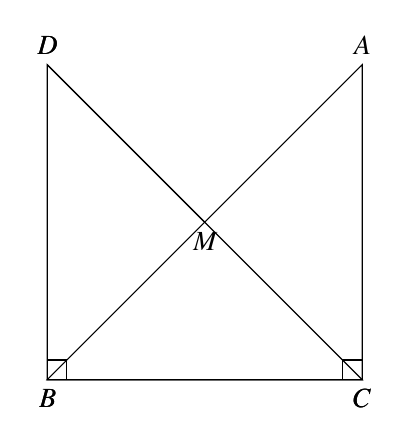
\begin{tikzpicture}
\coordinate (D) at (0,4);
\coordinate (A) at (4,4);
\coordinate (B) at (0,0);
\coordinate (C) at (4,0);
\coordinate (M) at (2,2);
\draw (A)node[above]{$A$}--(B)node[below]{$B$}--(C)node[below]{$C$}--cycle;
\draw (D)node[above]{$D$}--(B)node[below]{$B$}--(C)node[below]{$C$}--cycle;
\draw(M)node[below]{$M$}--(D)node[above]{$D$};
\tkzMarkRightAngle(D,B,C)
\tkzMarkRightAngle(A,C,B)
\end{tikzpicture}}
\caption{Triangle ABC and DBC}
\label{myfig}
\end{figure}
In $\triangle{ABC}$, $\vec{M}$ is midpoint of hypotenuse AB, thus 
\begin{align}
&\vec{M} = \frac{\vec{A}+\vec{B}}{2}\label{eq1} \\
&2\vec{M} = \brak{\vec{A+B}}\\
&\brak{\vec{A-M}} = \brak{\vec{M-B}}\\
&\norm{\vec{A}-\vec{M}}=\norm{\vec{M}-\vec{B}}\label{eq4} \\
&\vec{M} = \frac{\vec{C}+\vec{D}}{2}\label{eq2} \\
&2\vec{M} = \brak{\vec{C+D}}\\
&\brak{\vec{C-M}} = \brak{\vec{M-D}}\\
&\norm{\vec{C}-\vec{M}}=\norm{\vec{M}-\vec{D}}\label{eq5} \\
&\vec{M} = \frac{\vec{A}+\vec{B}}{2} = \frac{\vec{C}+\vec{D}}{2}\label{eq3} \\
&\vec{A - C} = \vec{A - M} + \vec{M - C} \\
&\vec{A - C} = \vec{M - B} + \vec{D - M} \\
&(\vec{A - C}) = k(\vec{D - B})\label{eq6} \quad\text{[k value is 1]}
\end{align} 
Now from equation \eqref{eq6} we can say that 
\begin{align}
&AC \parallel DB\label{eq8} \\
&\norm{\vec{A - C}} = \norm{\vec{D - B}}\label{eq7} 
\end{align}
Now it is given that AC $\perp$ BC, using this we can prove that DB $\perp$ BC. 
\begin{align}
&(\vec A -\vec C)^T(\vec{B}-\vec{C}) = 0 \\
&(\vec A -\vec M +\vec M -\vec C)^T(\vec{B}-\vec{C}) = 0 \\
&(\vec M -\vec B +\vec D -\vec M)^T(\vec{B}-\vec{C}) = 0 \\
&(\vec D -\vec B)^T(\vec{B}-\vec{C}) = 0 \\
&\implies DB \perp BC \\
&\vec{A - B} = \vec{A - C}+\vec{C - B} \\
&\vec{A - B} = \vec{B - D}+\vec{C - B} \quad\text{[From \eqref{eq7}]} \\
&\vec{A - B} = \vec{C - D} \\
&\vec{A - B} = \vec{C - M}+ \vec{M - D} \\
&\vec{A - B} = \vec{C - M}+\vec{C - M} \quad\text{[From \eqref{eq5}]}
\end{align} 
\begin{align}
&\vec{A - B} = 2 (\vec{C - M}) \\
&\vec{C - M} = \frac{1}{2}(\vec{A - B}) \\
&\norm{\vec{C - M}} = \frac{1}{2}\norm{\vec{A - B}}\label{eqFin1}
\end{align}
Hence from \eqref{eqFin1} proved,\\CM = $\frac{1}{2}$ AB
\end{document}